\newpage
\chapter{Results}
\label{cha:Results}

In Figure \ref{img:all_training} the progress for the training of each model and dataset combination is shown. Losses
and validation metrics are also displayed.

% \begin{figure}[H]
%   \centering
%   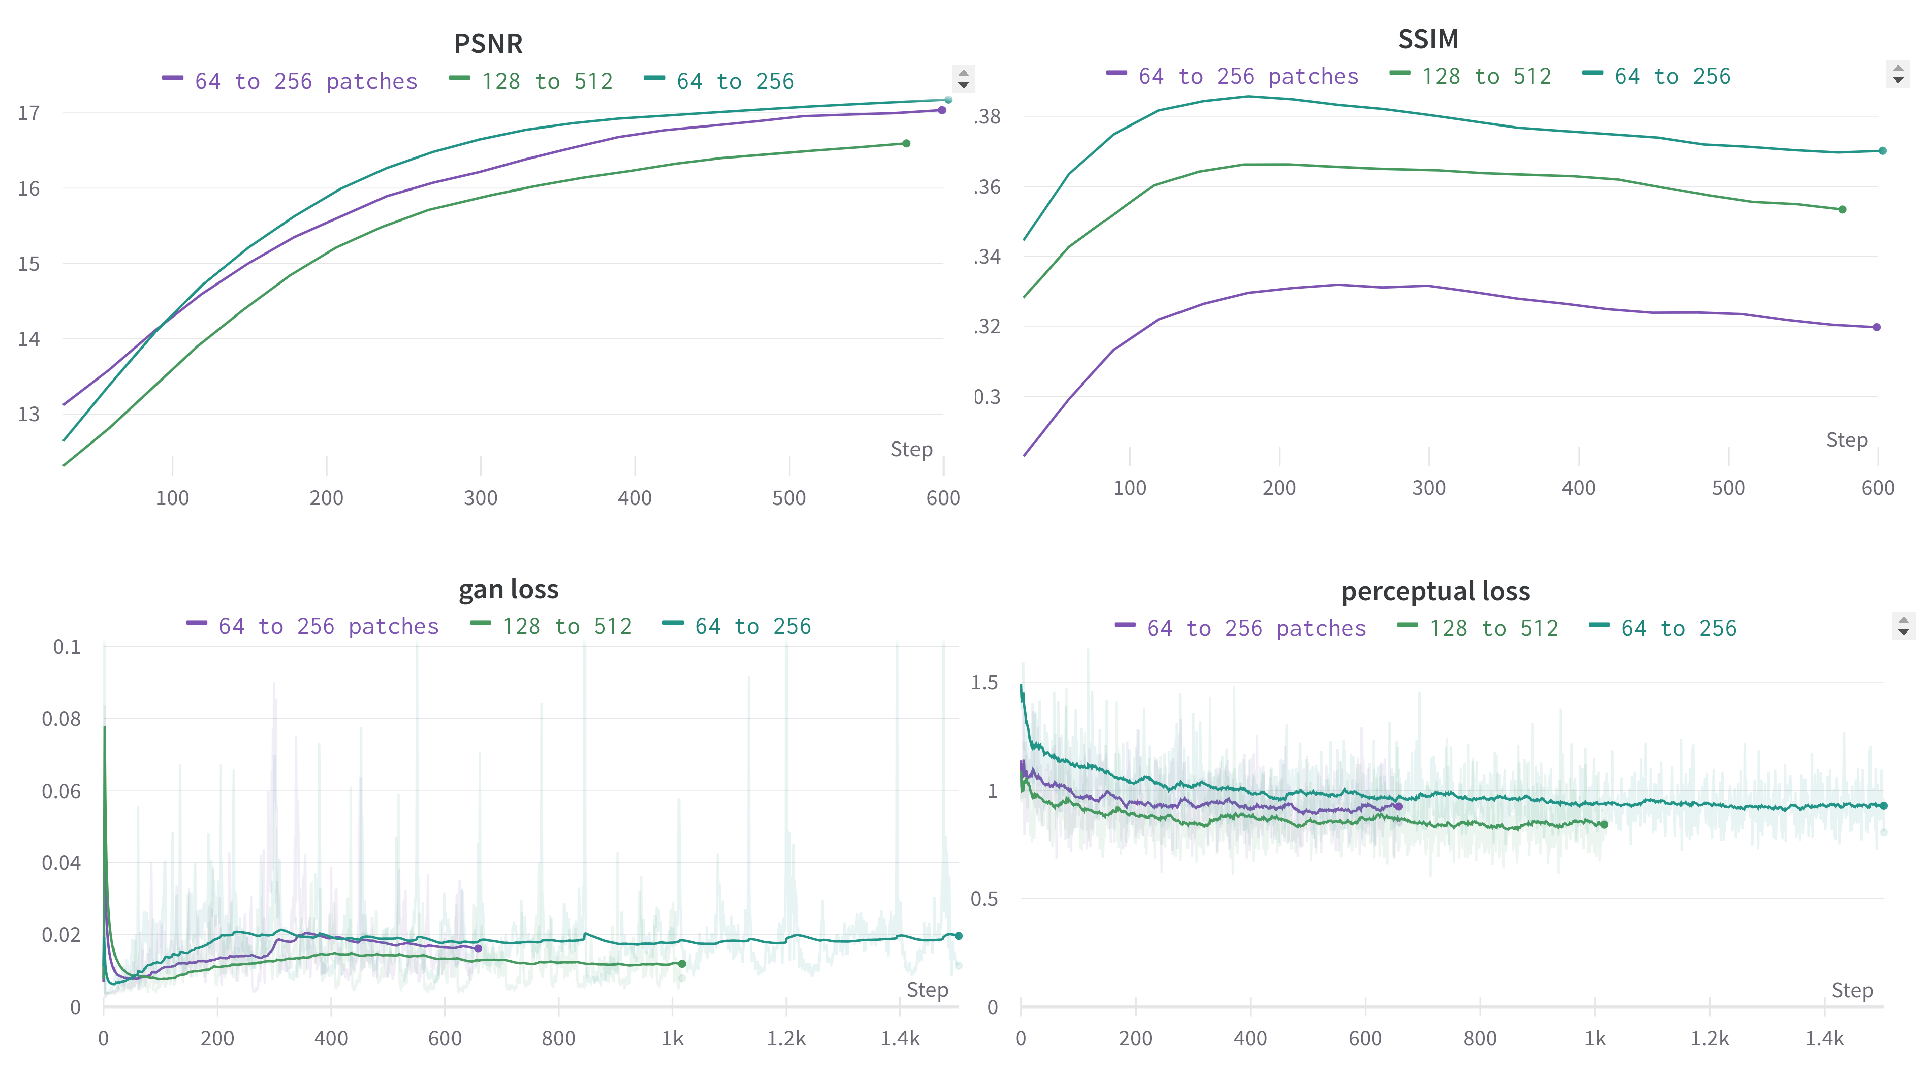
\includegraphics[scale=0.8]{figures/ESRGAN_compose.png}
%   \caption{PSNR, SSIM, gan loss and perceptual loss for ESRGAN over the training arch.}
%   \label{img:esrgan_training}
% \end{figure}

% \begin{figure}[H]
%   \centering
%   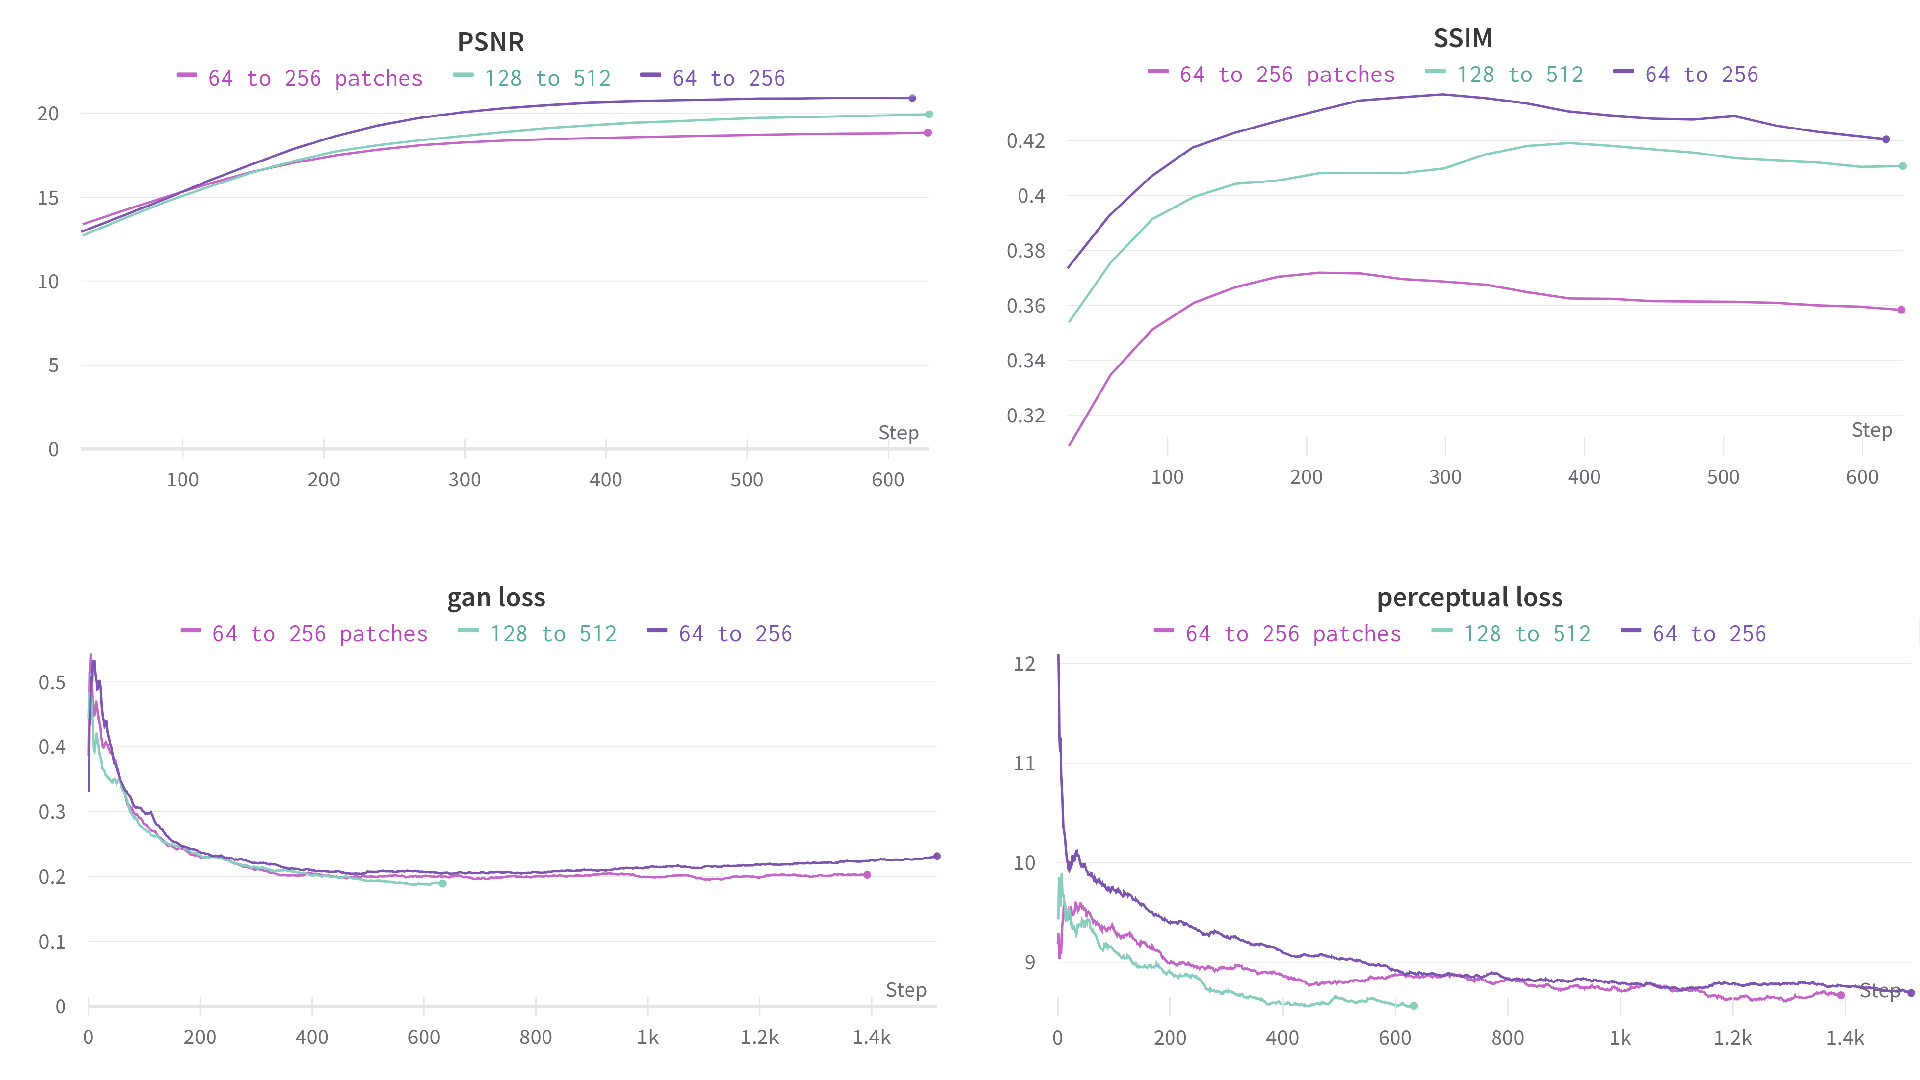
\includegraphics[scale=0.8]{figures/RealESRGAN_compose.png}
%   \caption{PSNR, SSIM, gan loss and perceptual loss for Real-ESRGAN over the training arch.}
%   \label{img:realesrgan_training}
% \end{figure}

% \begin{figure}[H]
%   \centering
%   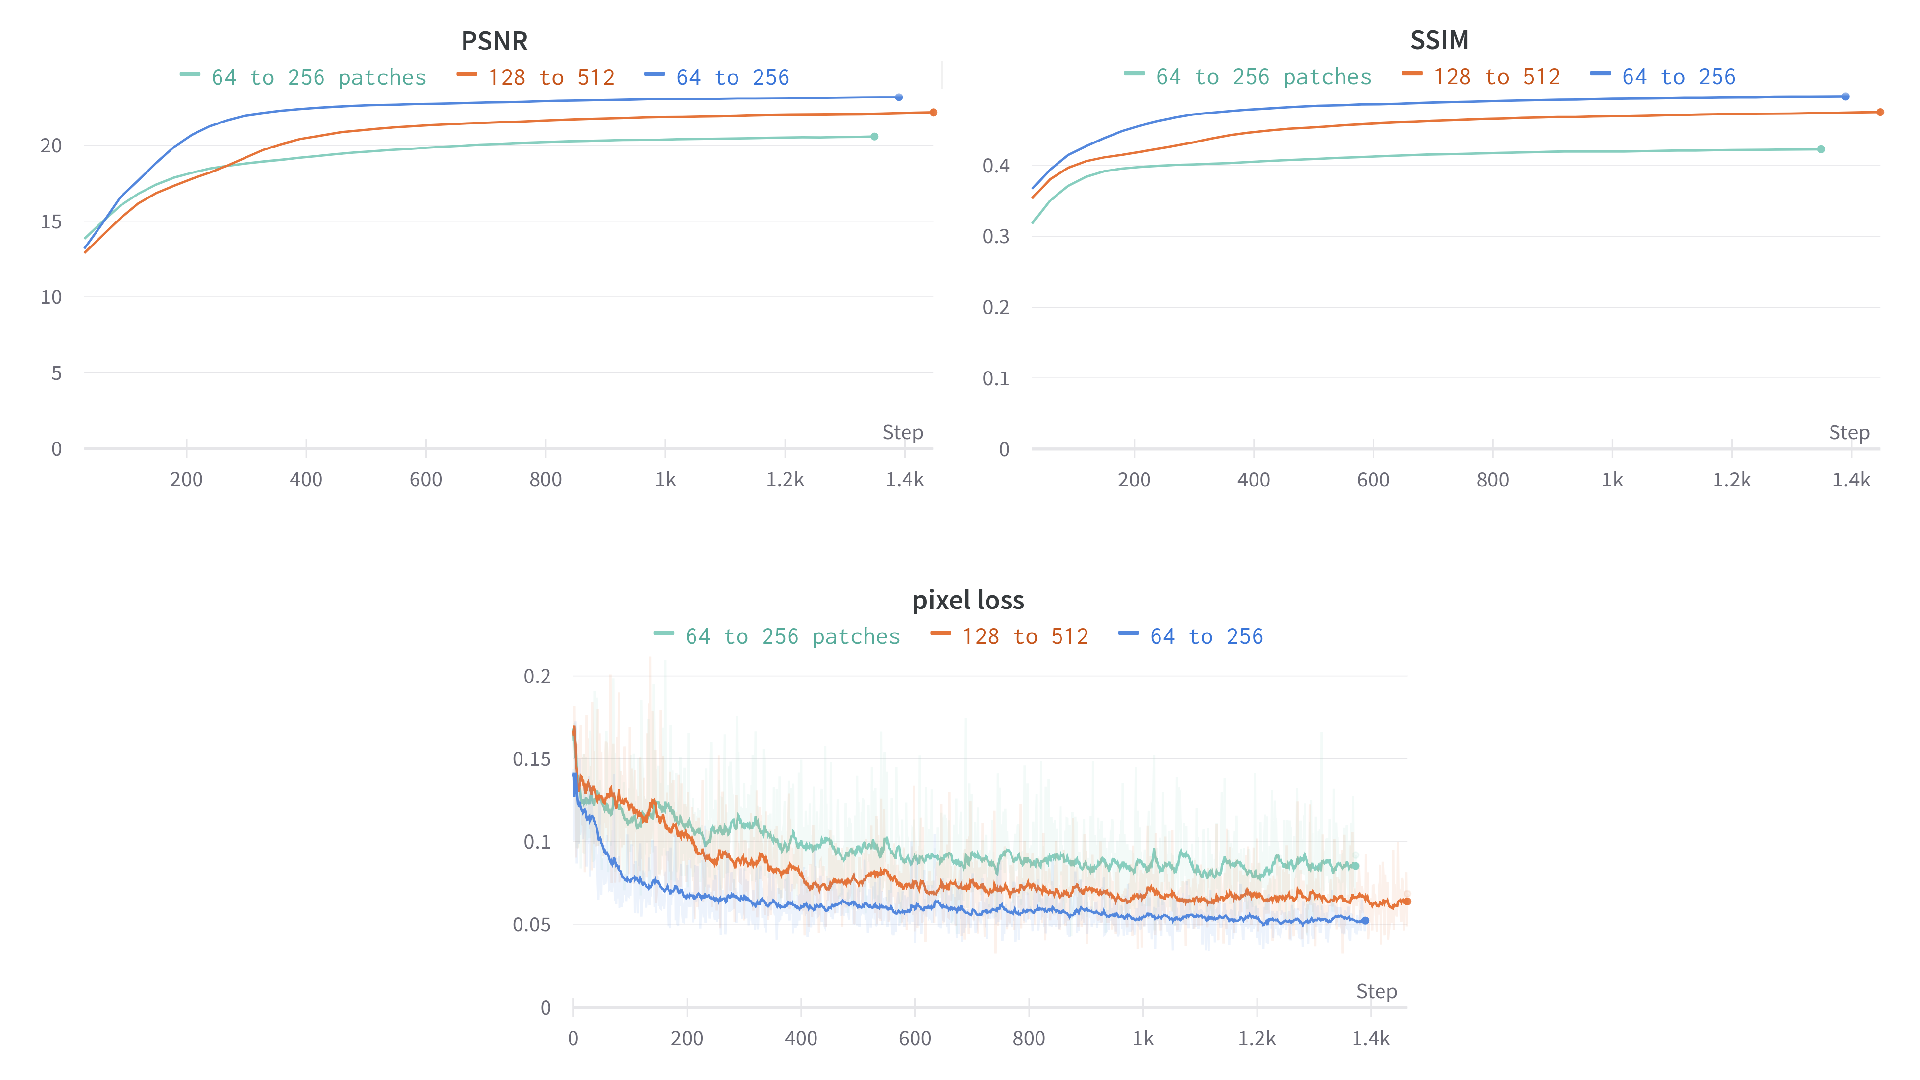
\includegraphics[scale=0.8]{figures/SwinIR_compose.png}
%   \caption{PSNR, SSIM and loss for SwinIR over the training arch.}
%   \label{img:swinir_training}
% \end{figure}

% \begin{figure}[H]
%   \centering
%   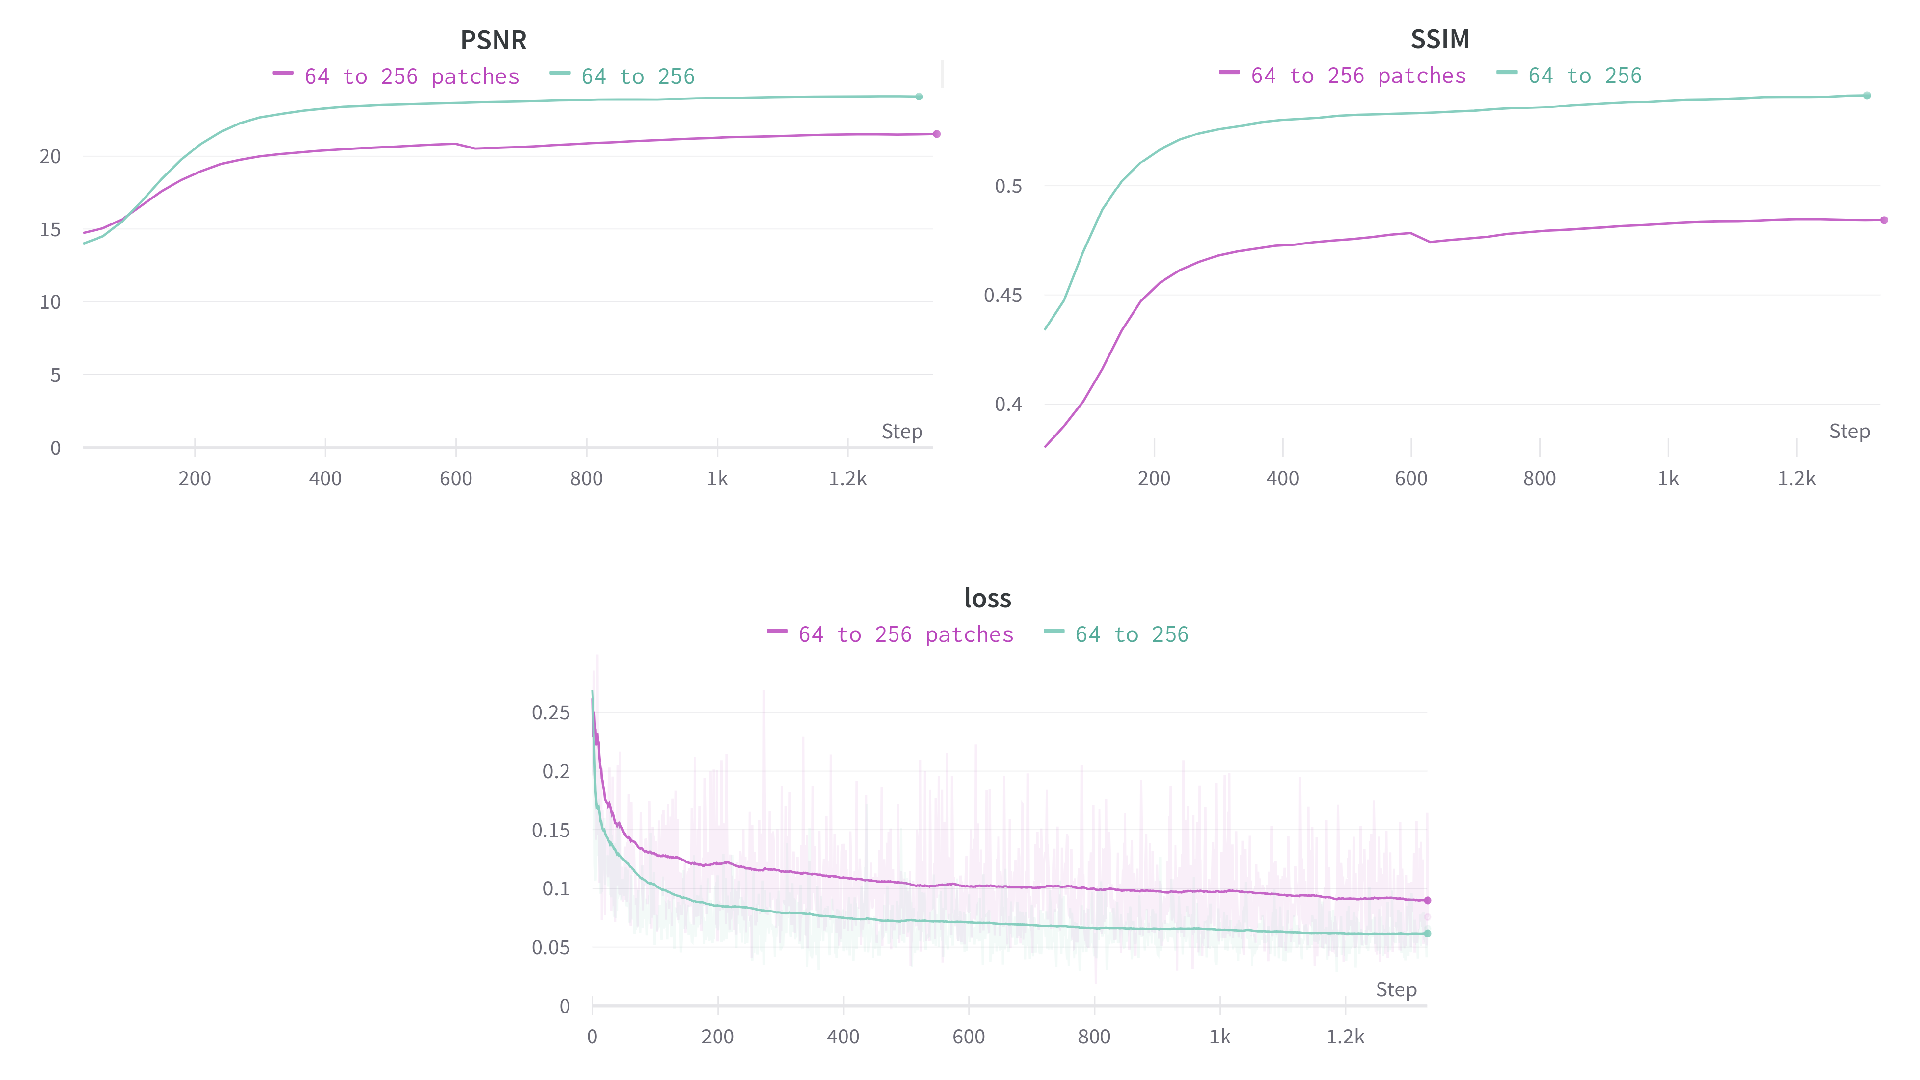
\includegraphics[scale=0.8]{figures/HATL_compose.png}
%   \caption{PSNR, SSIM and loss for HAT-L over the training arch.}
%   \label{img:hat_training}
% \end{figure}

\begin{figure}[H]
  \centering
  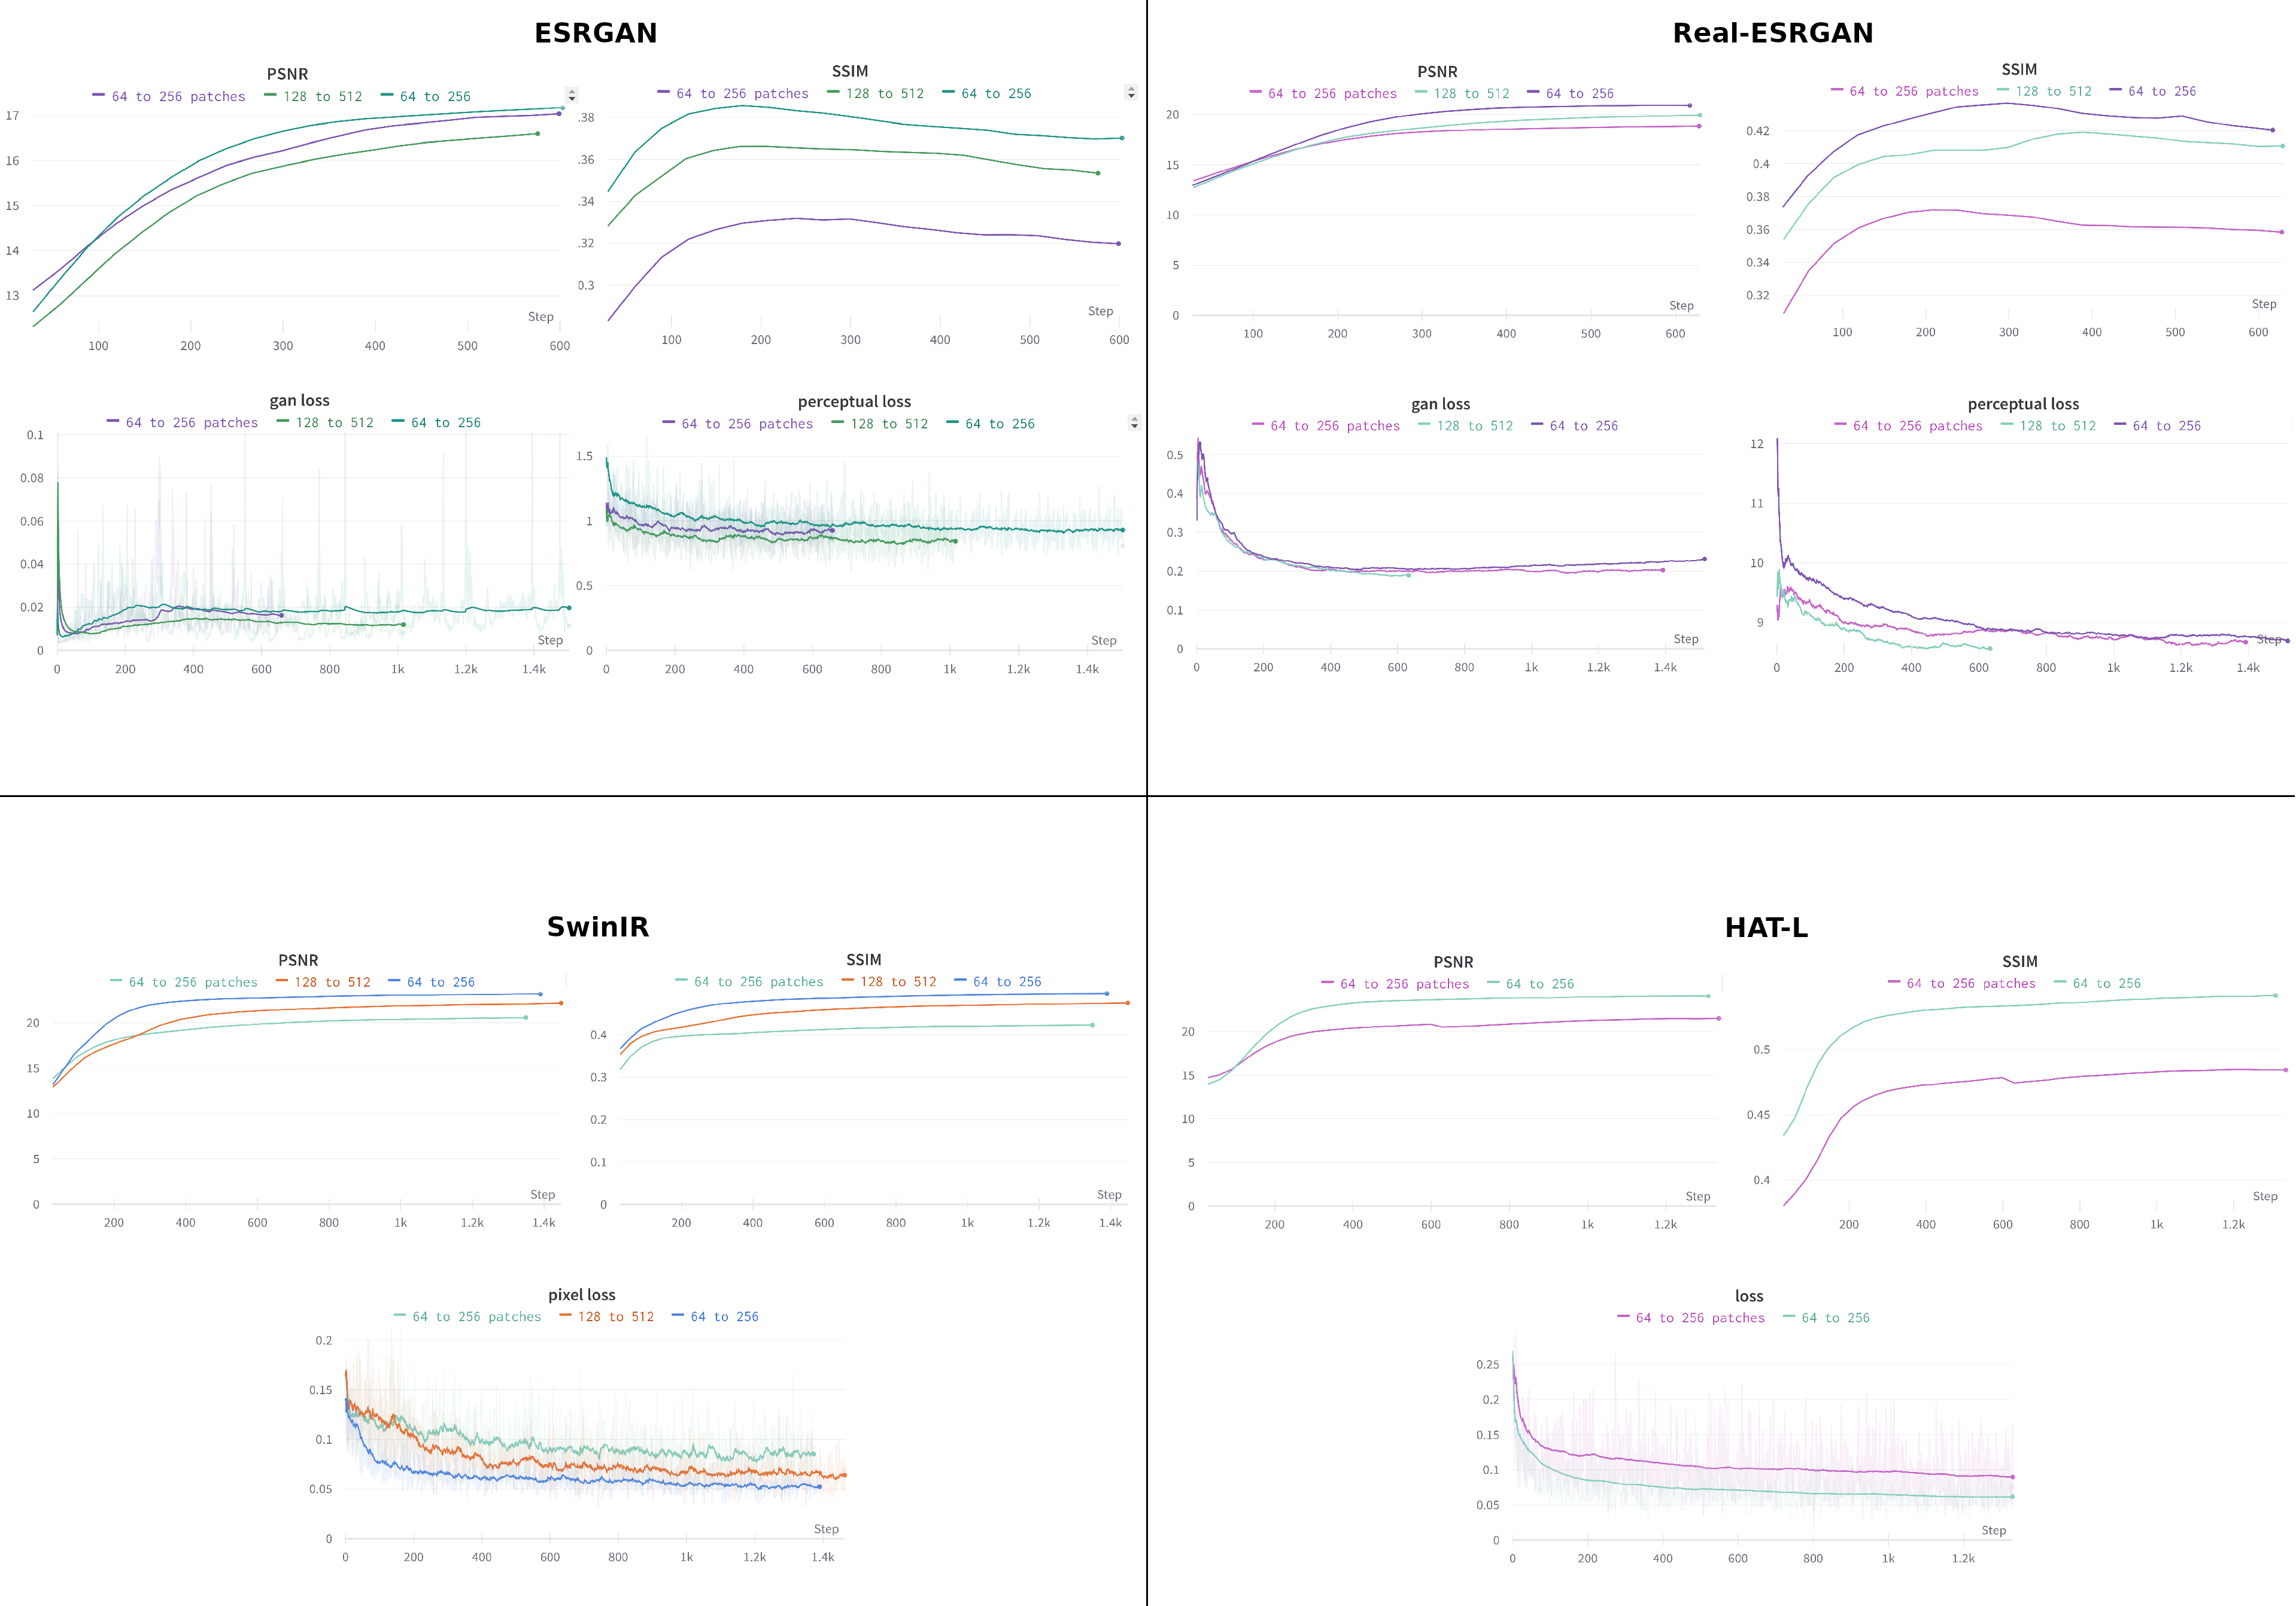
\includegraphics[scale=0.15,angle=90,origin=c]{figures/ALL_compose2.png}
  \caption{PSNR, SSIM and loss for all the models over the training arch.}
  \label{img:all_training}
\end{figure}

The models have been trained for up to 16k iterations (1 step equals 10 iterations), however from the graphs it's clear that in most cases that was much more than needed. ESRGAN and Real-ESRGAN show similar behavior, with PSNR steadily increasing and SSIM decreasing after around 2k to 3k iterations. HAT-L and SwinIR also had similar behaviours plateauing at around 5k iterations with results definitely better than their GAN-based counterparts. At first glance, the transformer-based model performed much better compared to the others, but the real surprise comes when checking the perceptual similarity metrics.

\section{Metrics and Inference}

\begin{figure}[H]
  \centering
  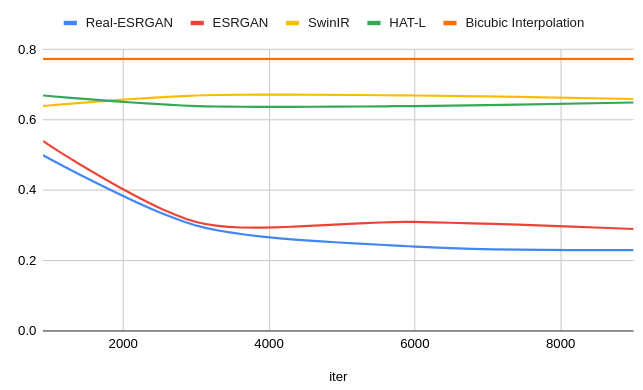
\includegraphics[scale=0.4]{figures/LPIPS_2.png}
  \caption{Comparisons of LPIPS metrics across bicubic interpolation and all models trained on the 64 to 256 dataset (lower is better).}
  \label{img:lpips}
\end{figure}


The disparity in performance between HAT-L and SwinIR, as opposed to Real-ESRGAN and the even more dated ESRGAN, is truly surprising when taking into account the much higher results scored by HAT-L and SwinIR in SSIM and PSNR. This phenomenon is evident in Figure \ref{img:lpips}, notably, the transformer-based models, HAT-L and SwinIR, exhibit a deteriorating trend in perceptual similarity over their training duration, in stark contrast ESRGAN and Real-ESRGAN show constant improvements for the entire arch of training. Table \ref{tab:metrics} provides a comprehensive array of metrics, offering a better understanding of the models' performances. This analysis includes Bicubic Interpolation as a baseline, serving as a reference point.


\begin{table}[H]
  \caption{Evaluated metrics for each combination of model and dataset, highlighted in red are the best results and in blue the second best. Bicubic interpolation is added as a baseline.}
  \label{tab:metrics}
  \begin{adjustbox}{max width=\textwidth}
  \begin{tabular}{c|ccc|ccc|ccc|}
  \cline{2-10}
  \rowcolor[HTML]{C0C0C0}
  \cellcolor[HTML]{FFFFFF}                                                                       & \multicolumn{3}{c|}{\cellcolor[HTML]{C0C0C0}\textbf{64 to 256}}                                                                                        & \multicolumn{3}{c|}{\cellcolor[HTML]{C0C0C0}\textbf{64 to 256 patches}}                                                                                & \multicolumn{3}{c|}{\cellcolor[HTML]{C0C0C0}\textbf{128 to 512}}                                                                                       \\ \hline
  \rowcolor[HTML]{C0C0C0}
  \multicolumn{1}{|c|}{\cellcolor[HTML]{C0C0C0}\textbf{Model}}                                   & \multicolumn{1}{c|}{\cellcolor[HTML]{C0C0C0}\textbf{PSNR}} & \multicolumn{1}{c|}{\cellcolor[HTML]{C0C0C0}\textbf{SSIM}} & \textbf{LPIPS}               & \multicolumn{1}{c|}{\cellcolor[HTML]{C0C0C0}\textbf{PSNR}} & \multicolumn{1}{c|}{\cellcolor[HTML]{C0C0C0}\textbf{SSIM}} & \textbf{LPIPS}               & \multicolumn{1}{c|}{\cellcolor[HTML]{C0C0C0}\textbf{PSNR}} & \multicolumn{1}{c|}{\cellcolor[HTML]{C0C0C0}\textbf{SSIM}} & \textbf{LPIPS}               \\ \hline
  \multicolumn{1}{|c|}{\textbf{ESRGAN}}                                                          & \multicolumn{1}{c|}{16.981}                                & \multicolumn{1}{c|}{0.369}                                 & {\color[HTML]{3531FF} 0.288} & \multicolumn{1}{c|}{16.328}                                & \multicolumn{1}{c|}{0.317}                                 & {\color[HTML]{3531FF} 0.361} & \multicolumn{1}{c|}{16.34}                                 & \multicolumn{1}{c|}{0.344}                                 & {\color[HTML]{3531FF} 0.353} \\ \hline
  \multicolumn{1}{|c|}{\textbf{Real-ESRGAN}}                                                     & \multicolumn{1}{c|}{20.392}                                & \multicolumn{1}{c|}{0.408}                                 & {\color[HTML]{FE0000} 0.225} & \multicolumn{1}{c|}{17.761}                                & \multicolumn{1}{c|}{0.355}                                 & {\color[HTML]{FE0000} 0.319} & \multicolumn{1}{c|}{{\color[HTML]{3531FF} 19.436}}         & \multicolumn{1}{c|}{{\color[HTML]{3531FF} 0.408}}          & {\color[HTML]{FE0000} 0.307} \\ \hline
  \multicolumn{1}{|c|}{\textbf{SwinIR}}                                                          & \multicolumn{1}{c|}{{\color[HTML]{FE0000} 22.46}}          & \multicolumn{1}{c|}{{\color[HTML]{FE0000} 0.492}}          & 0.667                        & \multicolumn{1}{c|}{{\color[HTML]{FE0000} 19.18}}          & \multicolumn{1}{c|}{{\color[HTML]{FE0000} 0.417}}          & 0.761                        & \multicolumn{1}{c|}{{\color[HTML]{FE0000} 21.25}}          & \multicolumn{1}{c|}{{\color[HTML]{FE0000} 0.466}}          & 0.696                        \\ \hline
  \multicolumn{1}{|c|}{\textbf{HAT-L}}                                                           & \multicolumn{1}{c|}{{\color[HTML]{3531FF} 21.63}}          & \multicolumn{1}{c|}{{\color[HTML]{3531FF} 0.478}}          & 0.651                        & \multicolumn{1}{c|}{{\color[HTML]{3531FF} 18.71}}          & \multicolumn{1}{c|}{{\color[HTML]{3531FF} 0.409}}          & 0.684                        & \multicolumn{1}{c|}{/}                                     & \multicolumn{1}{c|}{/}                                     & /                            \\ \hline
  \multicolumn{1}{|l|}{\textbf{\begin{tabular}[c]{@{}l@{}}Bicubic\\ Interpolation\end{tabular}}} & \multicolumn{1}{l|}{11.82}                                 & \multicolumn{1}{l|}{0.354}                                 & \multicolumn{1}{l|}{0.774}   & \multicolumn{1}{l|}{11.76}                                 & \multicolumn{1}{l|}{0.287}                                 & \multicolumn{1}{l|}{0.717}   & \multicolumn{1}{l|}{11.71}                                 & \multicolumn{1}{l|}{0.332}                                 & \multicolumn{1}{l|}{0.735}   \\ \hline
  \end{tabular}
  \end{adjustbox}
  \end{table}

Although already present in the validation metrics, both PSNR and SSIM have been measured again along LPIPS for more consistent results and a better leveled field.

The results in Table \ref{tab:metrics} have been evaluated taking into consideration for each combination of model and dataset the checkpoint with best performance.
With that model, each LR image of the validation set has been supersampled and analyzed with its corresponding ground truth (GT), once recorded the evalutaion outcome for each pair or supersampled image and high resolution GT the totals were averaged over the entire set and saved. Unlike for the results in Figure \ref{img:all_training}, the implementation of SSIM and PSNR used in Table \ref{tab:metrics} is not the one provided directly by BasicSR but we used Torchmetrics' implementation, the LPIPS implementation comes from the original library \cite{lpips2}.


The best and second-best score for each metric are highlighted respectively in red and blue. While SwinIR outperformed all the other models in both PSNR and SSIM and HAT-L comes a close second in the same metrics, Real-ESRGAN and ESRGAN showed the best results overall for perceptual similarity with a good margin on the transformer-based models.


\begin{figure}[H]

  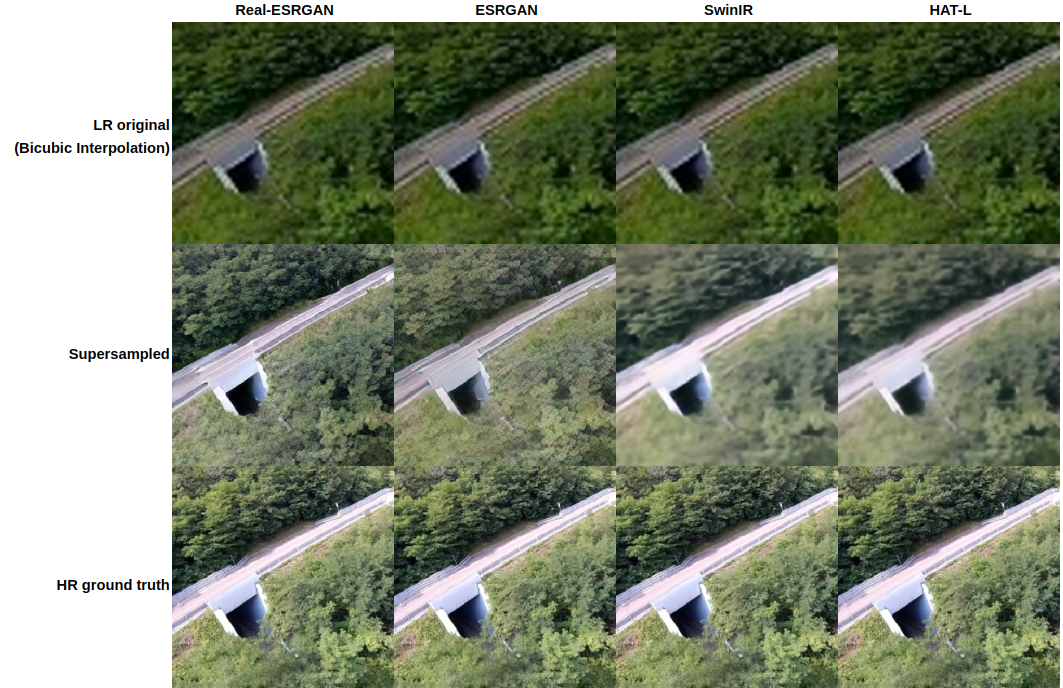
\includegraphics[width=1\textwidth]{figures/results/comp_table.png}
  \caption{Final results compared side by side.}
  \label{img:comp_table}
\end{figure}

In Figure \ref{img:comp_table} is even clearer the reason for good perceptual similarity scores in Real-ESRGAN and ESRGAN: the supersampled images from HAT-L and SwinIR look blurred while the other two are sharp with fine details and defined edges.

Although the networks behaved very differently the results of Real-ESRGAN and ESRGAN are very pleasing, not only the models are able to create sharp and realistic images but they also learned extremely well to transfer the style of the HR camera to the LR frames, mimicing color balance and even exposure to a satistactory degree.

\begin{figure}[H]
  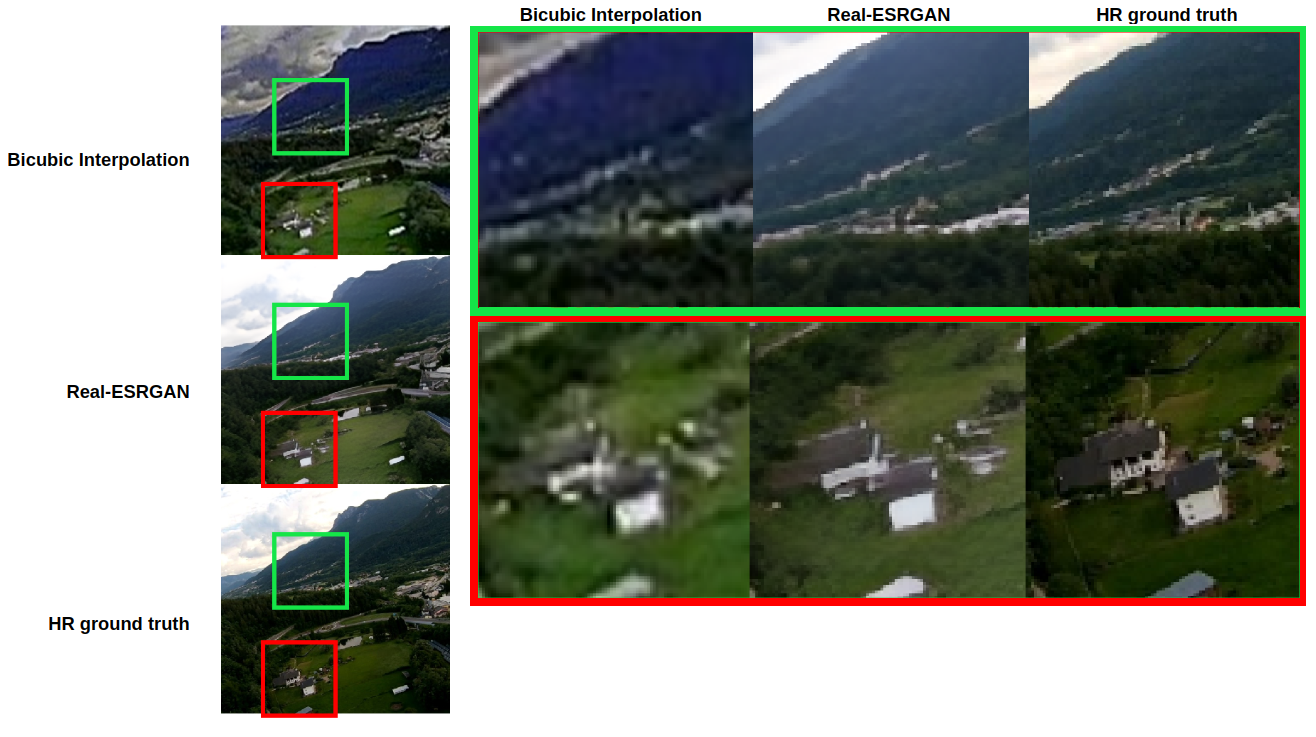
\includegraphics[width=1\textwidth]{figures/results/realesrgan128_example_table.png}
  \caption{Details of a supersampled \(128\times128\) frame.}
  \label{img:example_table}
\end{figure}

In Figure \ref{img:example_table} some details of a \(128\times128\) frame supersampled to \(512\times512\) using Real-ESRGAN are highlighted. Even though some details are lost in the process, it can be noted that the quality of the image in much higher compared to a shallow bicubic interpolation and the style is very close to the one of the high-resolution camera. More supersampled examples for all the models are present in the appendix.
